\documentclass[9pt,twoside,lineno]{pnas-new}
% Use the lineno option to display guide line numbers if required.

\templatetype{pnassupportinginfo}

% Math
\def\P{\mathbb{P}}
\def\cor{\mathrm{cor}}
\def\Quantile{\mathrm{Quantile}}
\def\logit{\mathrm{logit}}
\def\dist{\mathrm{dist}}
\def\WIS{\mathrm{WIS}}
\def\AUC{\mathrm{AUC}}
\newcommand{\indicator}[1]{\mathbf{1}\left(#1\right)}

% Figures and tables
\usepackage{xurl}
\usepackage{microtype}
\usepackage{booktabs}
\usepackage{caption}
\usepackage{subcaption}
\usepackage{xcolor}
\newcommand{\attn}[1]{\textcolor{red}{[ATTN: #1]}}

\makeatletter 
\renewcommand\@biblabel[1]{#1} 
\makeatother

% indicators
\newcommand{\chngcli}{CHNG-CLI}
\newcommand{\chngcov}{CHNG-COVID}
\newcommand{\dv}{DV-CLI}
\newcommand{\ar}{AR}
\newcommand{\fb}{CTIS-CLI-in-community}
\newcommand{\gs}{Google-AA}


\providecommand{\tightlist}{%
  \setlength{\itemsep}{0pt}\setlength{\parskip}{0pt}}


\title{Your main manuscript title}
\author{Author1, Author2 and Author3 (complete author list)}
\correspondingauthor{Corresponding Author name.\\E-mail: author.two@email.com}

\begin{document}

%% Comment out or remove this line before generating final copy for submission; this will also remove the warning re: "Consecutive odd pages found".
\instructionspage  

\maketitle

%% Adds the main heading for the SI text. Comment out this line if you do not have any supporting information text.
\SItext


\section*{PNAS Template material, to be removed}

\subsection*{Subhead}
Type or paste text here. This should be additional explanatory text such as an extended technical description of results, full details of mathematical models, etc.   

\section*{Heading}
\subsection*{Subhead}
Type or paste text here. You may break this section up into subheads as needed (e.g., one section on ``Materials'' and one on ``Methods'').

\subsection*{Materials}
Add a materials subsection if you need to.

\subsection*{Methods}
Add a methods subsection if you need to.


%%% Each figure should be on its own page
\begin{figure}
\centering
\includegraphics[width=\textwidth]{example-image}
\caption{First figure}
\end{figure}

\begin{figure}
\centering
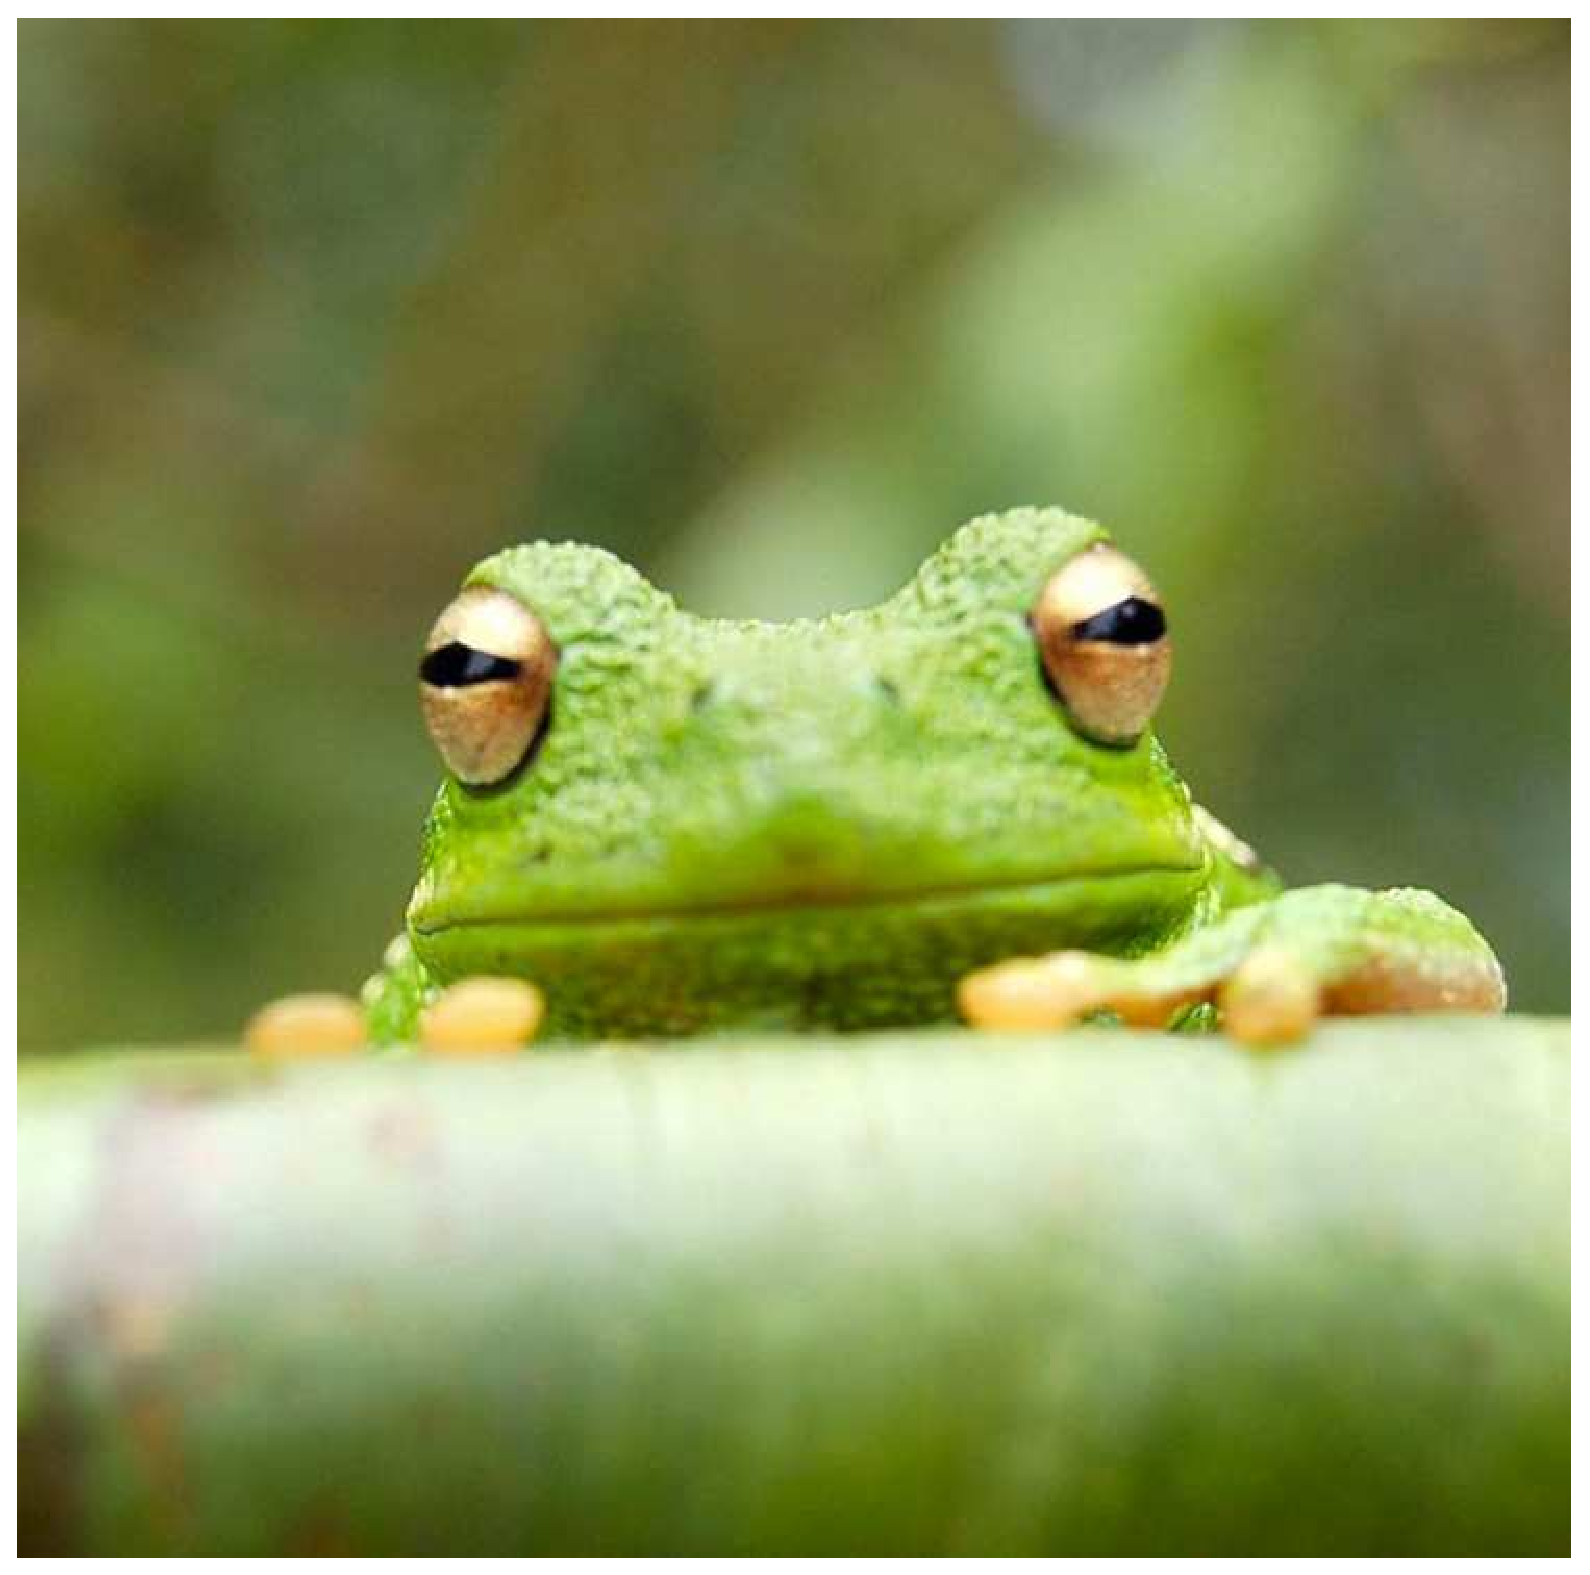
\includegraphics[width=\textwidth]{pnas-materials/frog}
\caption{Second figure}
\end{figure}

\begin{table}\centering
\caption{This is a table}

\begin{tabular}{lrrr}
Species & CBS & CV & G3 \\
\midrule
1. Acetaldehyde & 0.0 & 0.0 & 0.0 \\
2. Vinyl alcohol & 9.1 & 9.6 & 13.5 \\
3. Hydroxyethylidene & 50.8 & 51.2 & 54.0\\
\bottomrule
\end{tabular}
\end{table}


\clearpage

\hypertarget{figures-from-results}{%
\section{Figures from results}\label{figures-from-results}}

\hypertarget{forecasts}{%
\subsection{Forecasts}\label{forecasts}}

\begin{center}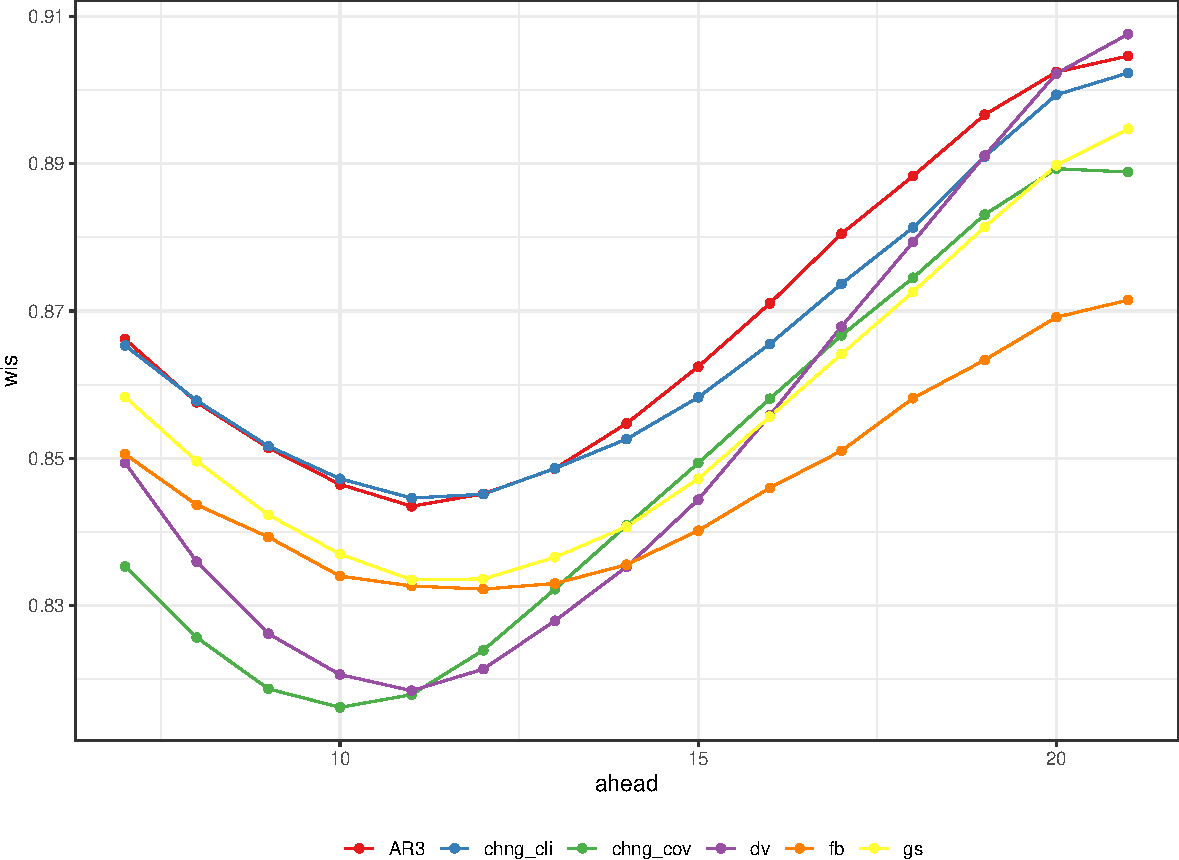
\includegraphics[width=\linewidth]{fig/fcast-1} \end{center}

\begin{center}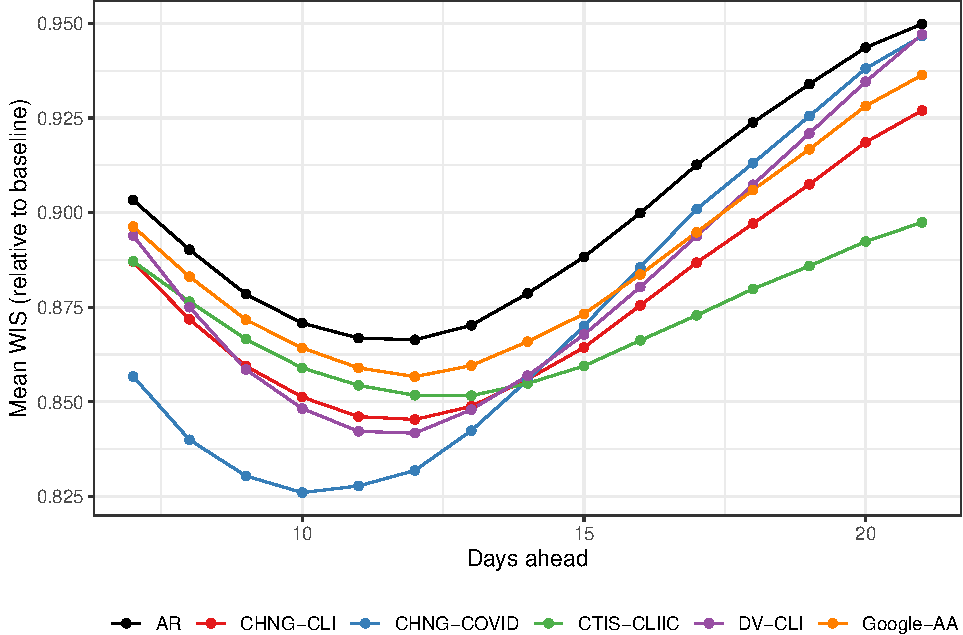
\includegraphics[width=\linewidth]{fig/fcast-finalized-1} \end{center}

\begin{center}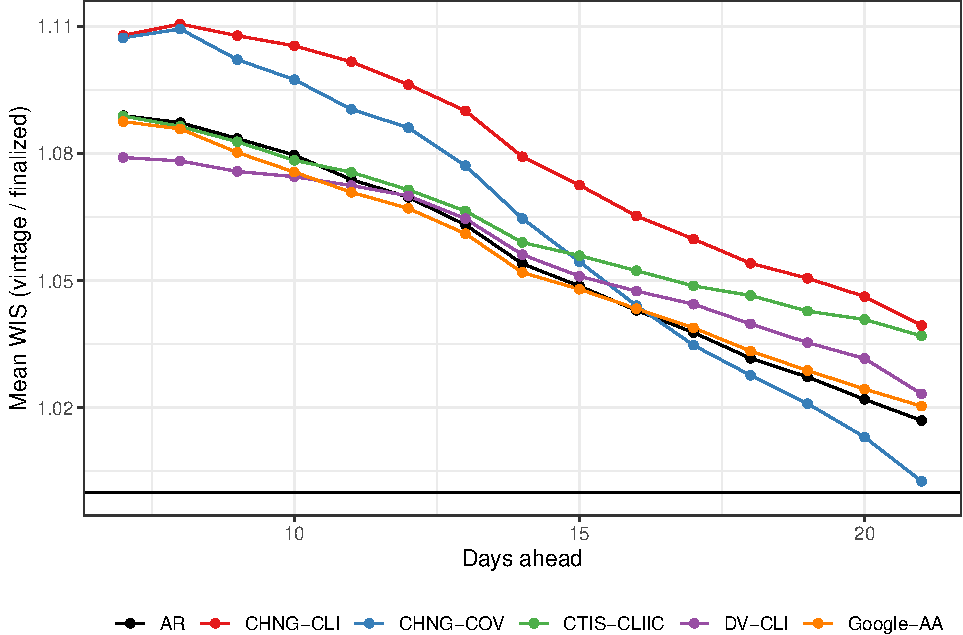
\includegraphics[width=\linewidth]{fig/fcast-honest-v-finalized-1} \end{center}

\begin{center}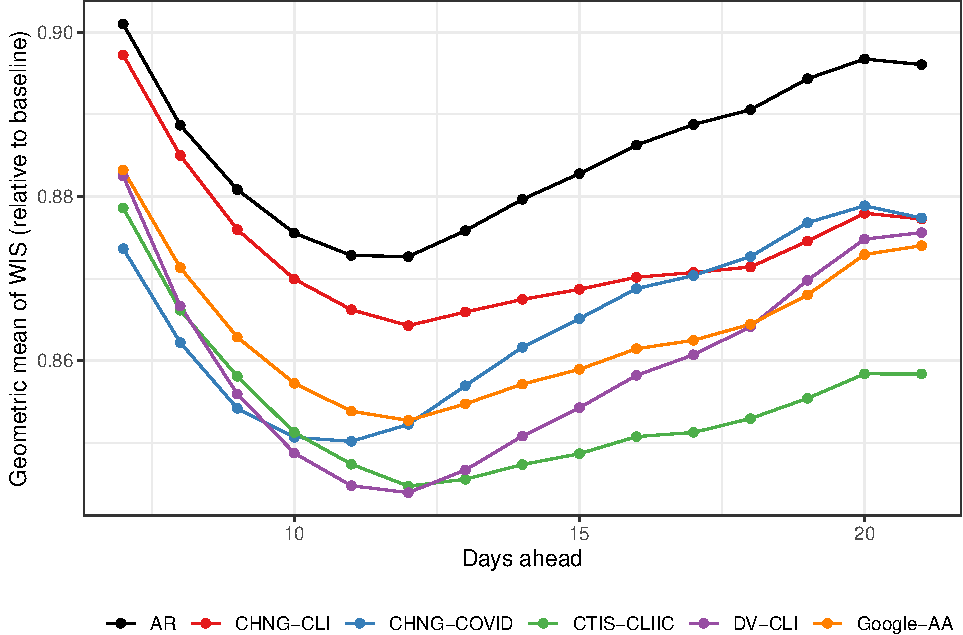
\includegraphics[width=\linewidth]{fig/fcast-adjusted-1} \end{center}

\begin{center}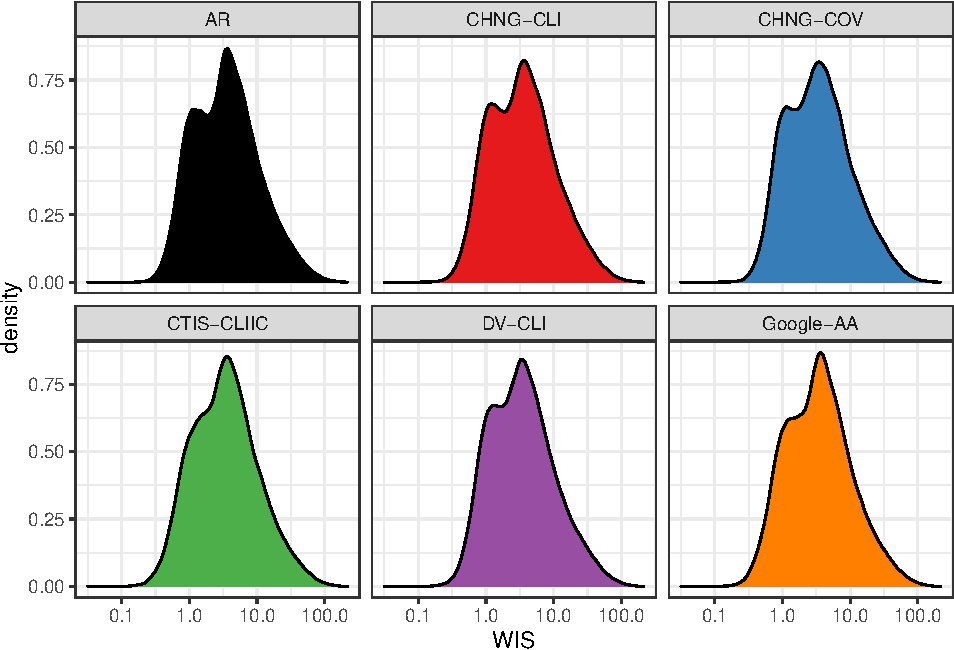
\includegraphics[width=\linewidth]{fig/wis-densities-1} \end{center}

\hypertarget{all-periods}{%
\subsubsection{All periods}\label{all-periods}}

\begin{center}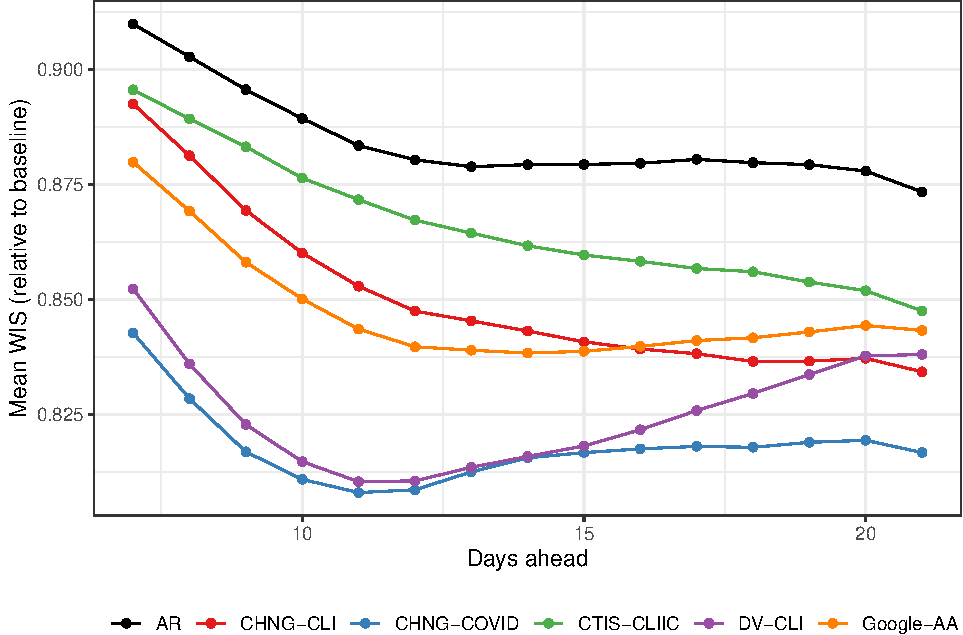
\includegraphics[width=\linewidth]{fig/fcast-alldates-1} \end{center}

\begin{center}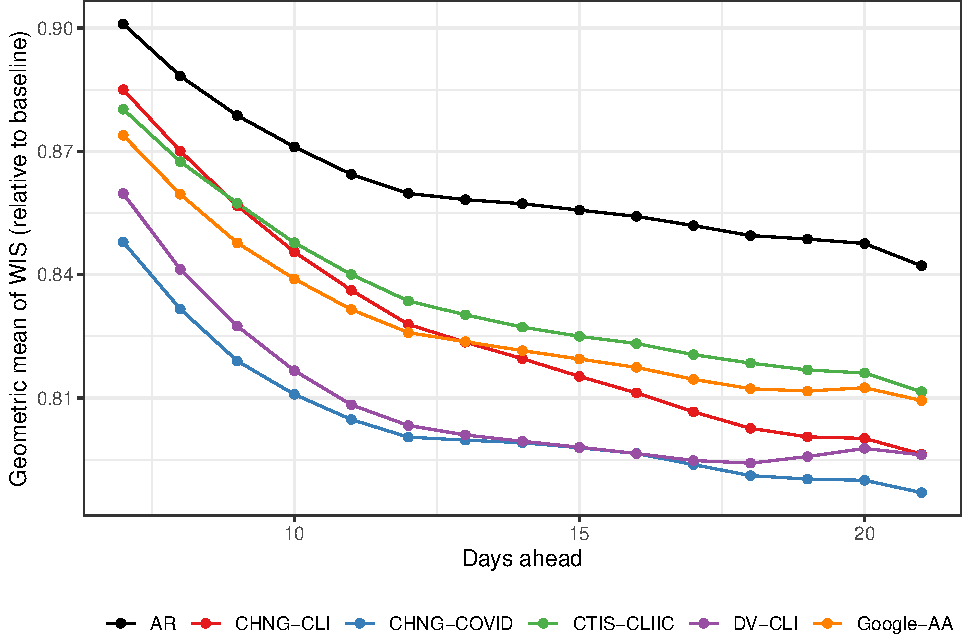
\includegraphics[width=\linewidth]{fig/fcast-alldates-adjusted-1} \end{center}

\hypertarget{only-gs-locations}{%
\subsubsection{Only GS locations}\label{only-gs-locations}}

\begin{center}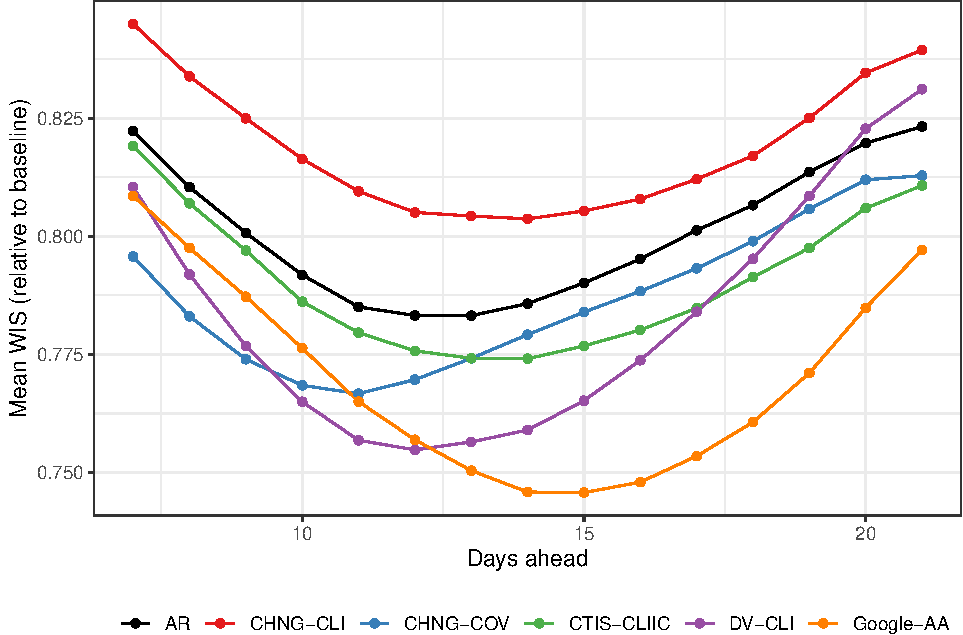
\includegraphics[width=\linewidth]{fig/fcast-gs-locations-1} \end{center}

\begin{center}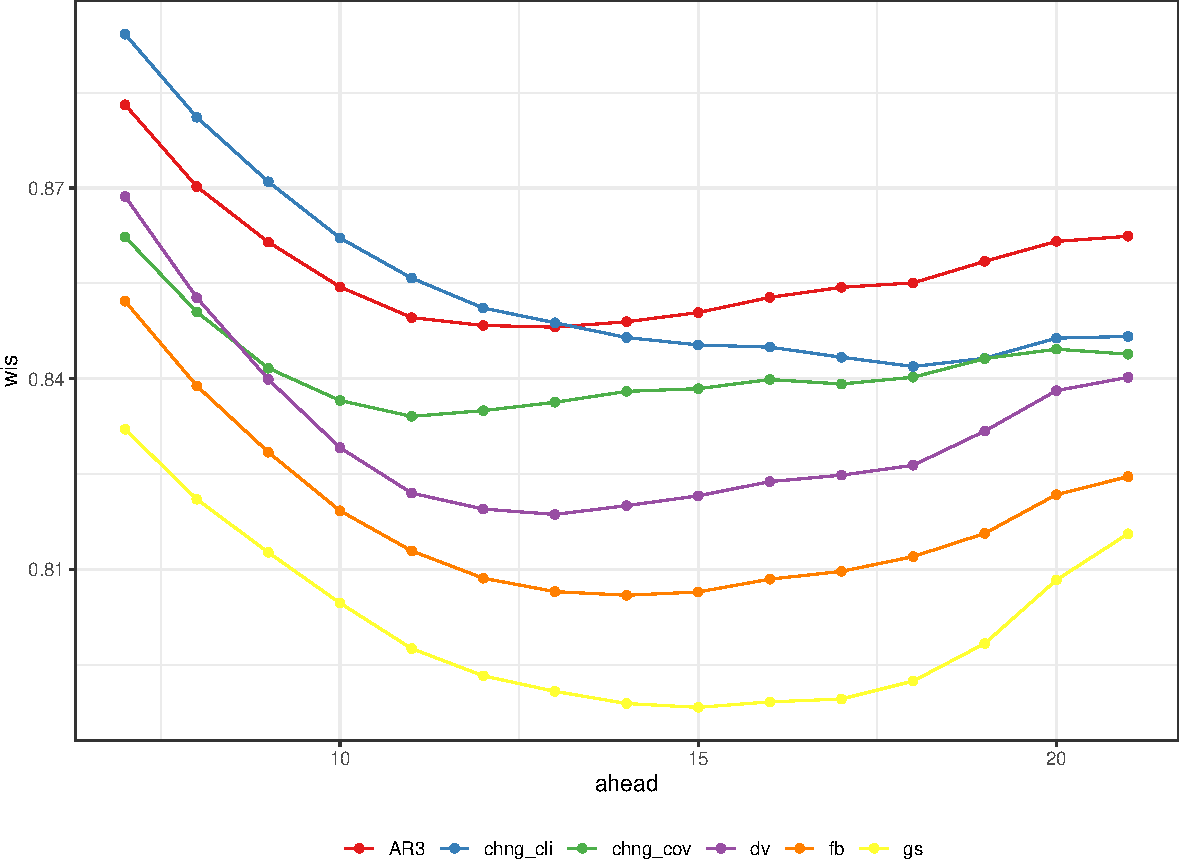
\includegraphics[width=\linewidth]{fig/fcast-gs-locations-adjusted-1} \end{center}

\hypertarget{trajectories-deprecated}{%
\subsection{Trajectories (deprecated)}\label{trajectories-deprecated}}

\hypertarget{hotspots}{%
\subsection{Hotspots}\label{hotspots}}

\begin{center}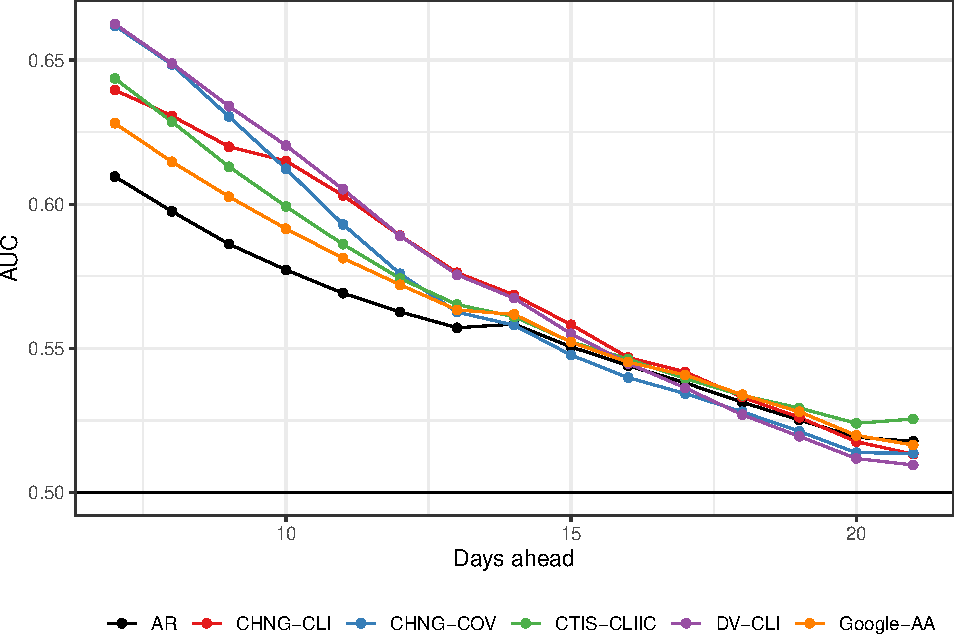
\includegraphics[width=\linewidth]{fig/hot-1} \end{center}

\begin{center}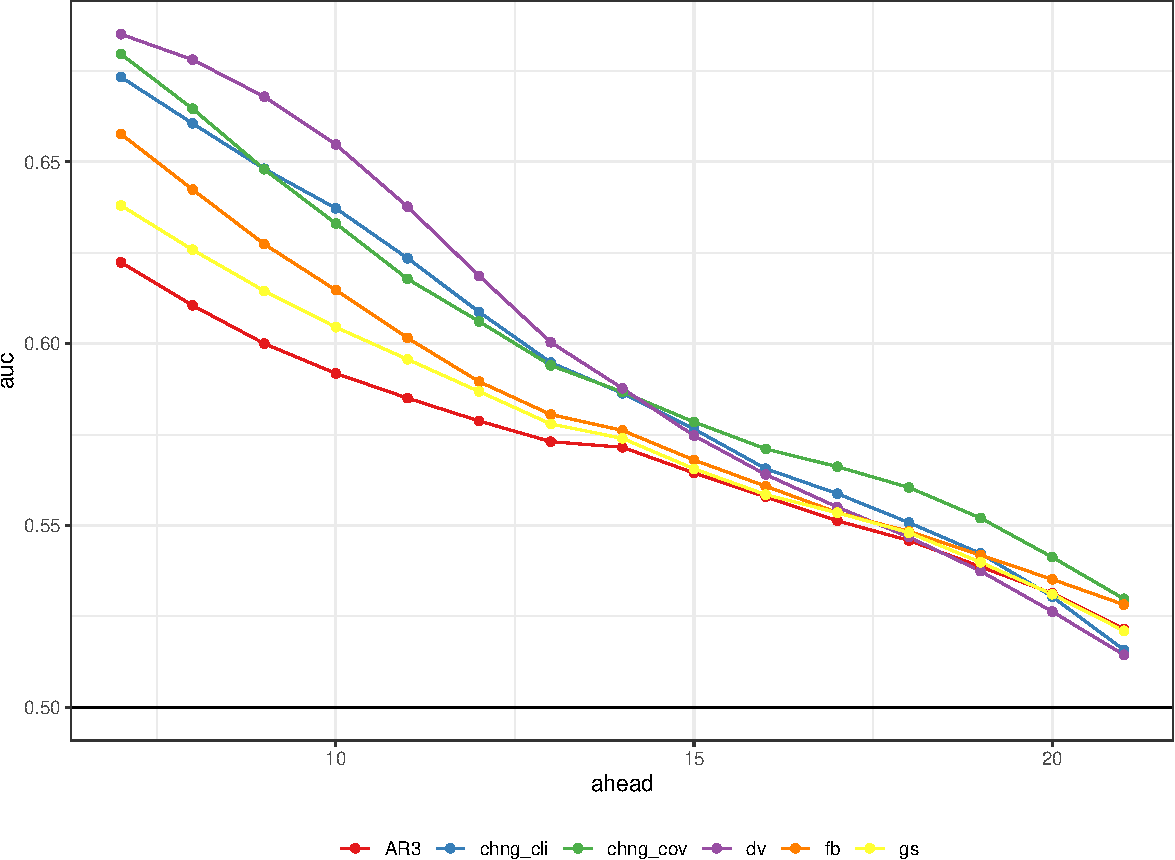
\includegraphics[width=\linewidth]{fig/hot-finalized-1} \end{center}

\begin{center}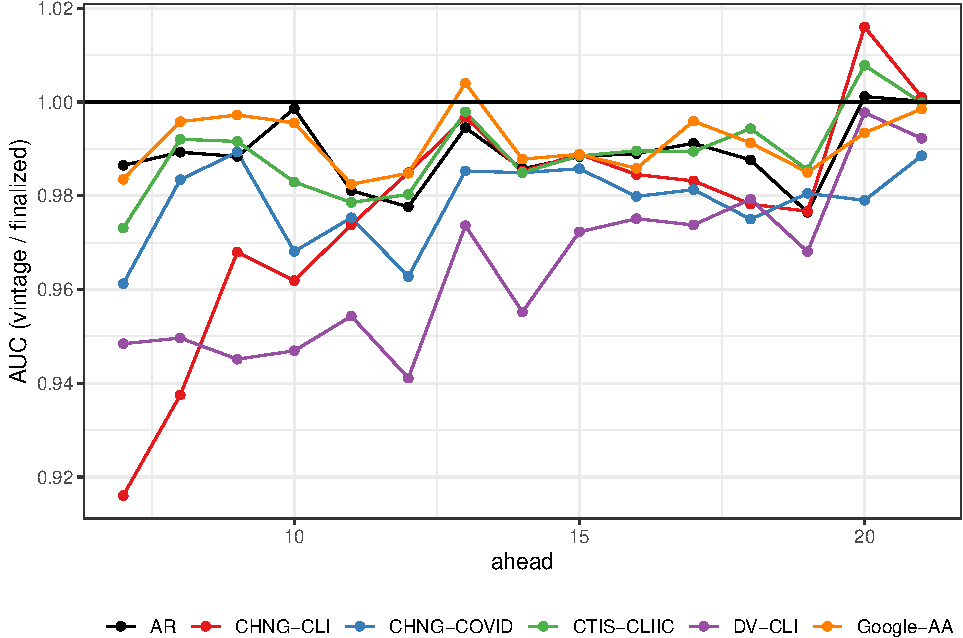
\includegraphics[width=\linewidth]{fig/hot-honest-v-finalized-1} \end{center}

\hypertarget{all-periods-1}{%
\subsubsection{All periods}\label{all-periods-1}}

\begin{center}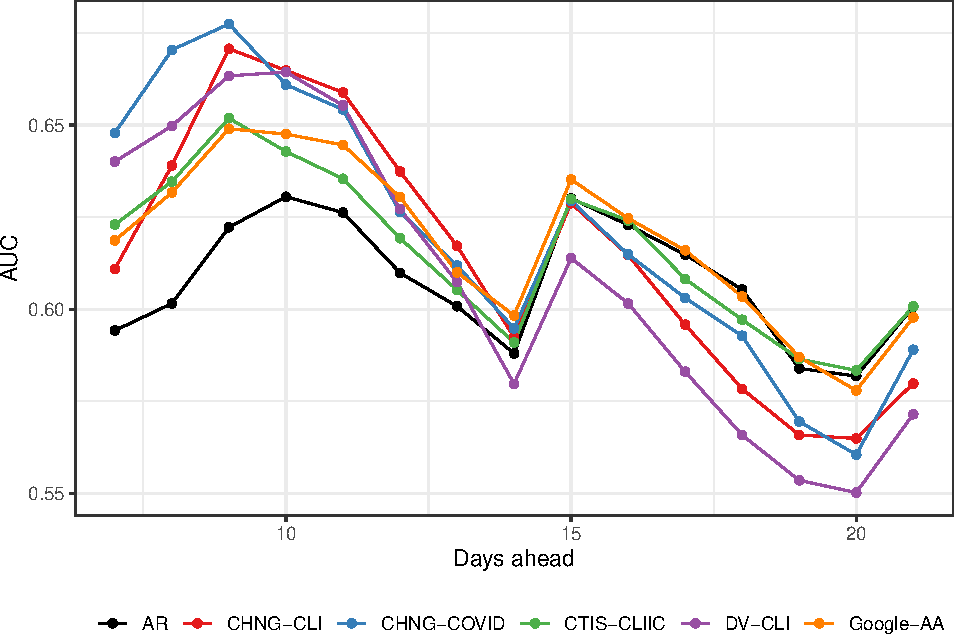
\includegraphics[width=\linewidth]{fig/hot-alldates-1} \end{center}

\hypertarget{only-gs-locations-1}{%
\subsubsection{Only GS locations}\label{only-gs-locations-1}}

\begin{center}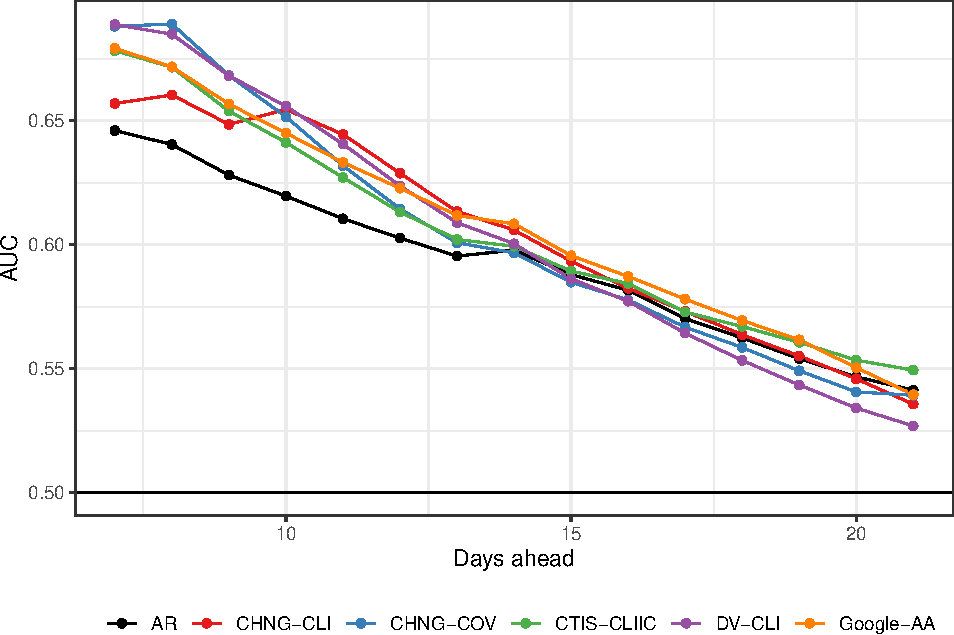
\includegraphics[width=\linewidth]{fig/hot-gs-locations-1} \end{center}

\hypertarget{figure-5}{%
\subsubsection{Figure 5}\label{figure-5}}

\begin{itemize}
\tightlist
\item
  Currently, this is the ``main'' figure. WIS and hotspots, 2 panels,
  only 2020, honest training.
\end{itemize}

\begin{center}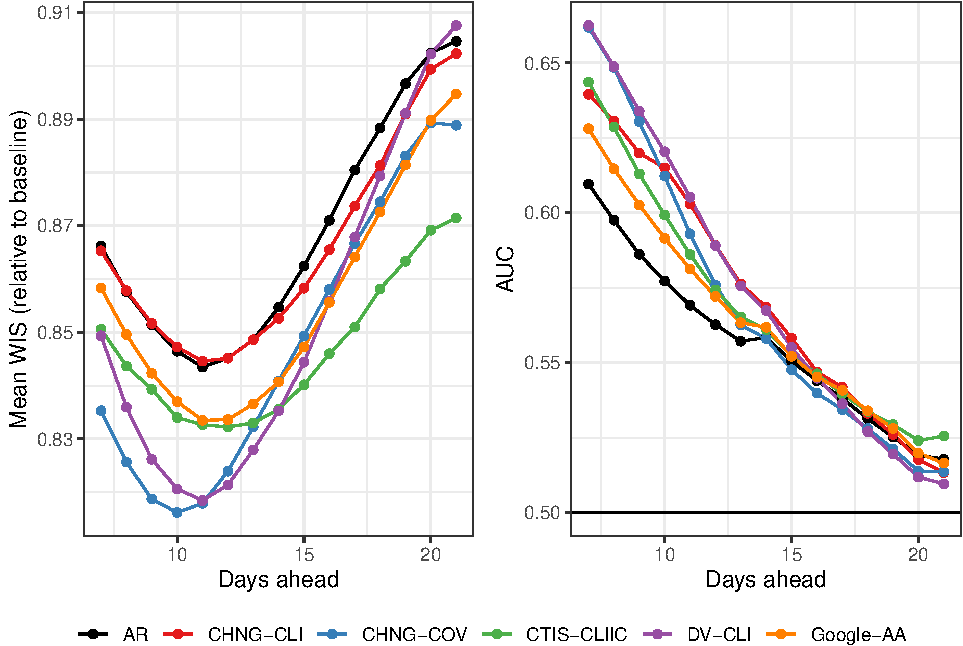
\includegraphics[width=\linewidth]{fig/figure5-1} \end{center}

\hypertarget{figure-6-misleading-retrospective-analysis}{%
\subsubsection{Figure 6 (misleading retrospective
analysis)}\label{figure-6-misleading-retrospective-analysis}}

\begin{itemize}
\tightlist
\item
  WIS and hotspots, 2 panels, only 2020, honest training.
\end{itemize}

\begin{center}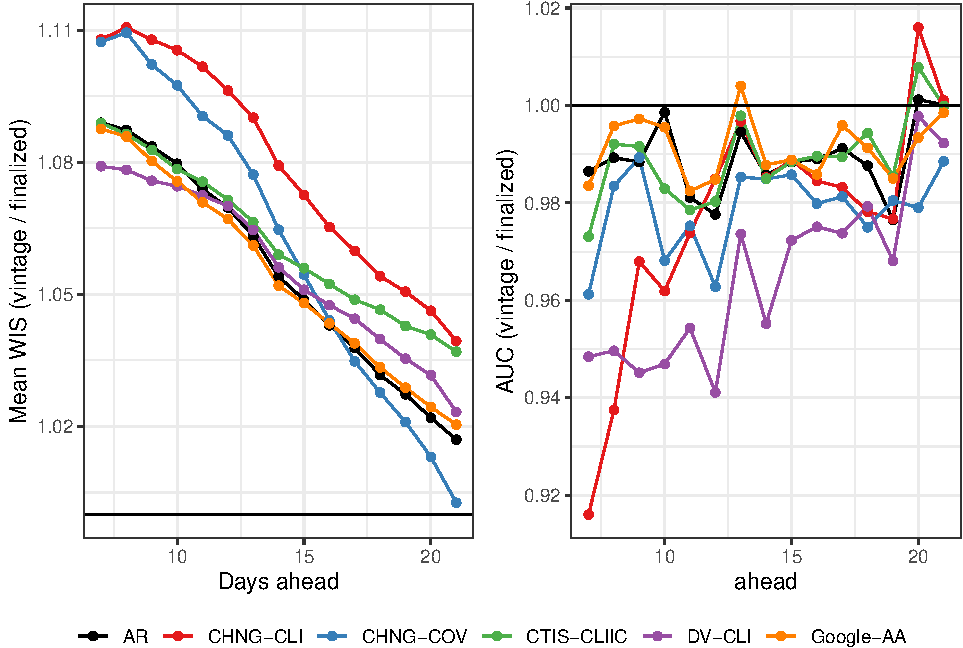
\includegraphics[width=\linewidth]{fig/figure6-1} \end{center}

\hypertarget{correlations-with-lagged-actuals}{%
\subsection{Correlations with lagged
actuals}\label{correlations-with-lagged-actuals}}

\begin{center}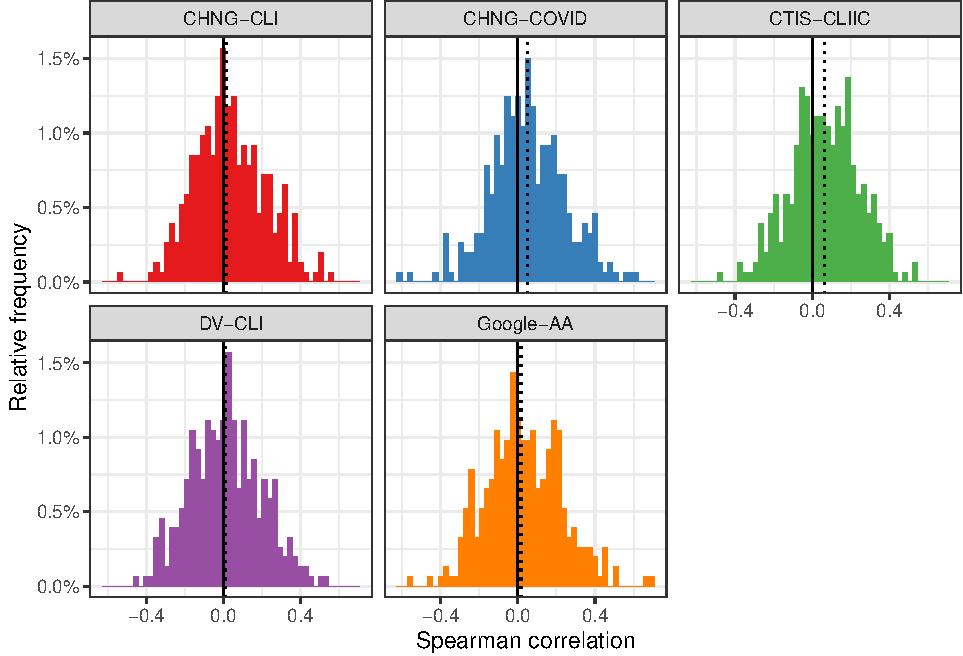
\includegraphics[width=\linewidth]{fig/cor-wis-ratio-1} \end{center}

\begin{center}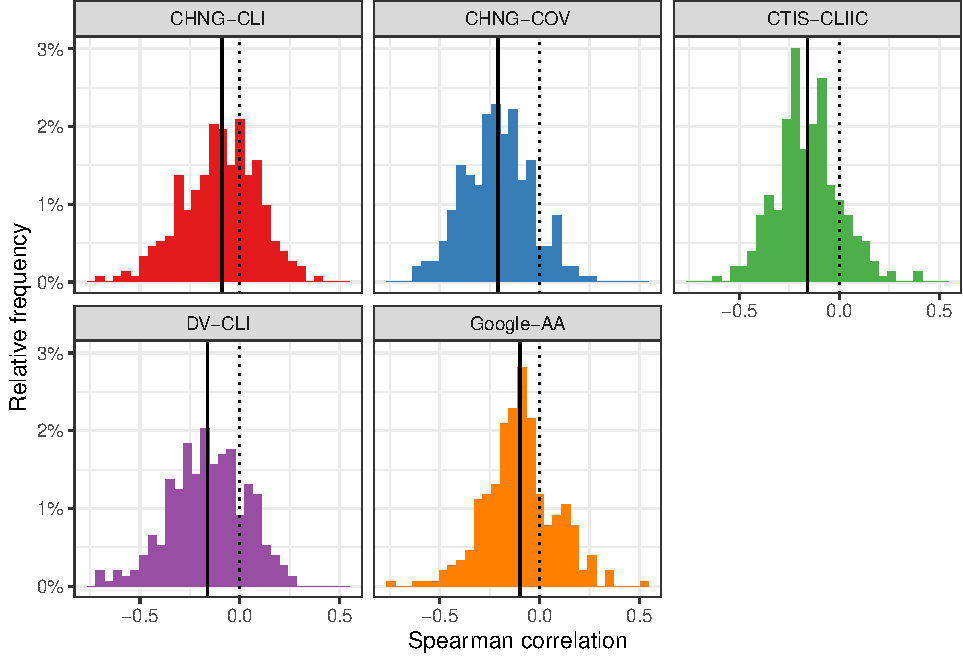
\includegraphics[width=\linewidth]{fig/cor-wis-ratio-m1-1} \end{center}

\hypertarget{upswings-vs-downswings}{%
\subsection{Upswings vs downswings}\label{upswings-vs-downswings}}

\begin{center}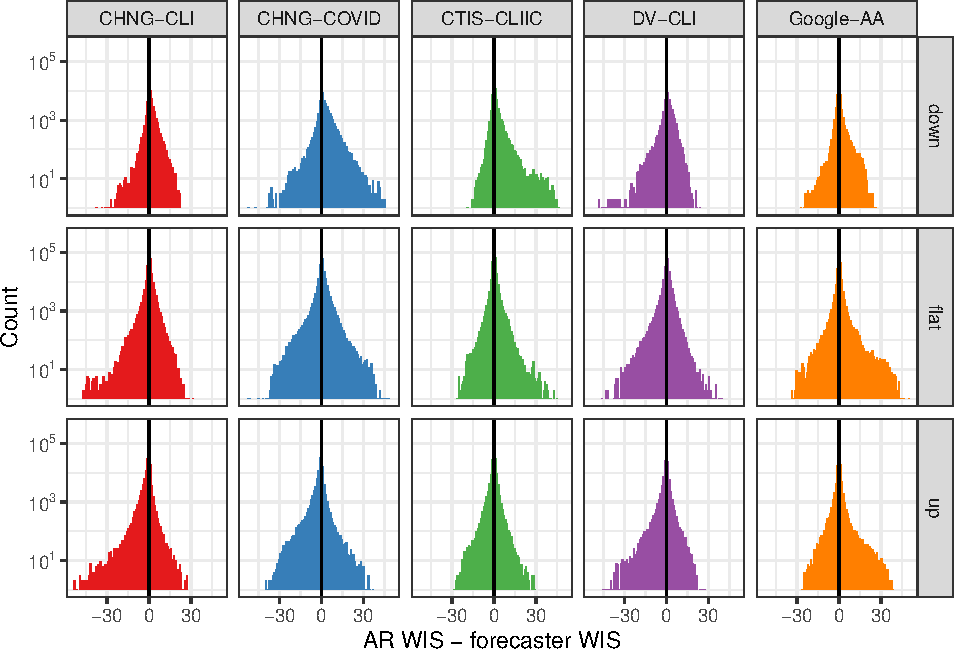
\includegraphics[width=\linewidth]{fig/upswing-histogram-1} \end{center}

\begin{center}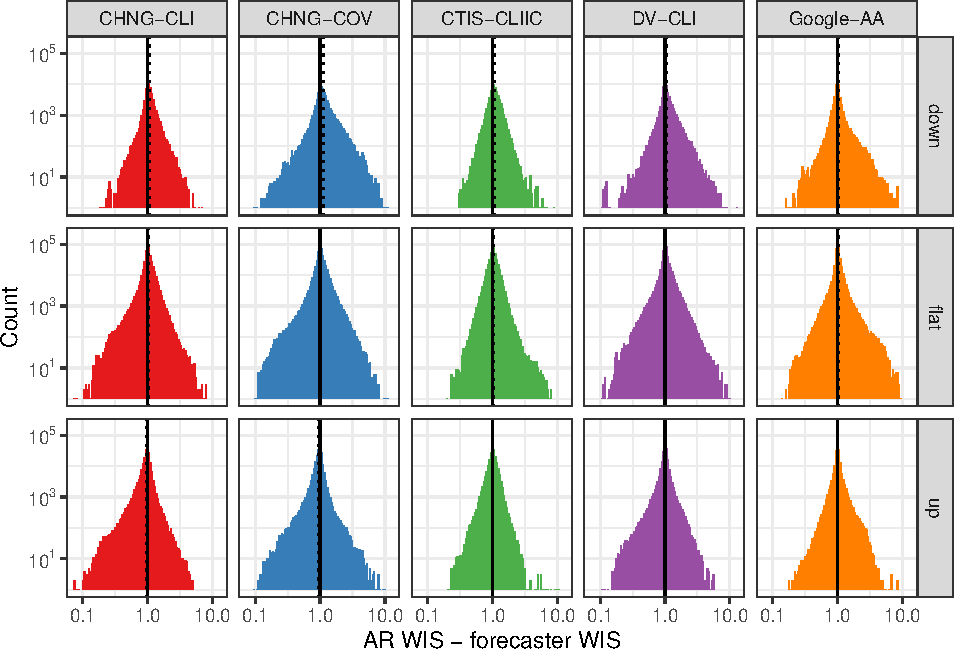
\includegraphics[width=\linewidth]{fig/upswing-histogram-logged-1} \end{center}

\begin{tabular}[t]{lrrrrr}
\toprule
udf & CHNG-CLI & CHNG-COV & CTIS-CLIIC & DV-CLI & Google-AA\\
\midrule
down & 0.79 & 0.80 & 0.83 & 0.81 & 0.81\\
flat & 0.12 & 0.17 & 0.28 & 0.18 & 0.17\\
up & -0.57 & -0.56 & -0.53 & -0.53 & -0.47\\
\bottomrule
\end{tabular}

\hypertarget{leadingness-and-laggingness}{%
\subsection{Leadingness and
laggingness}\label{leadingness-and-laggingness}}

\begin{center}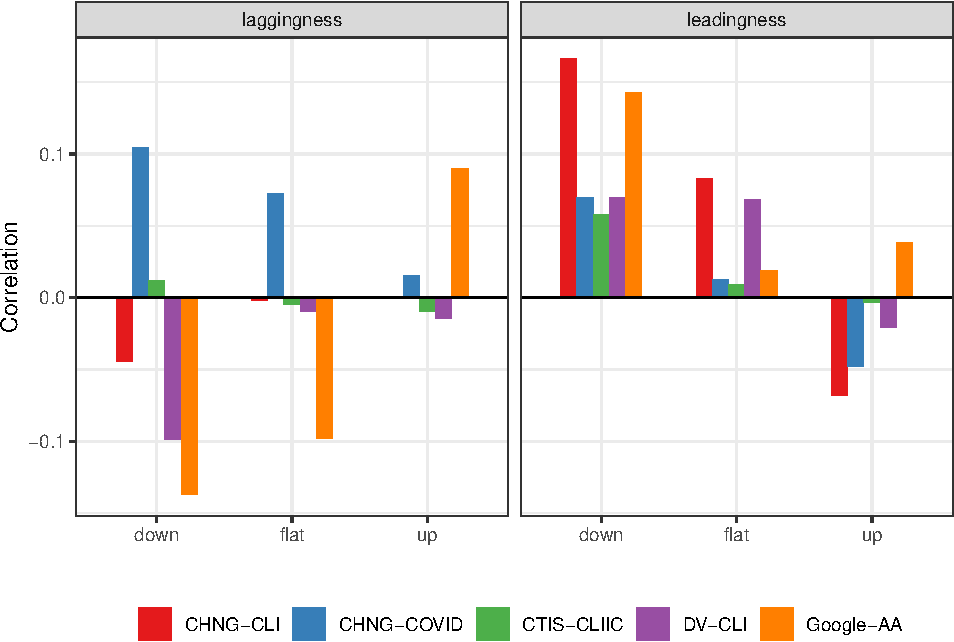
\includegraphics[width=\linewidth]{fig/leading-and-lagging-1} \end{center}

\begin{center}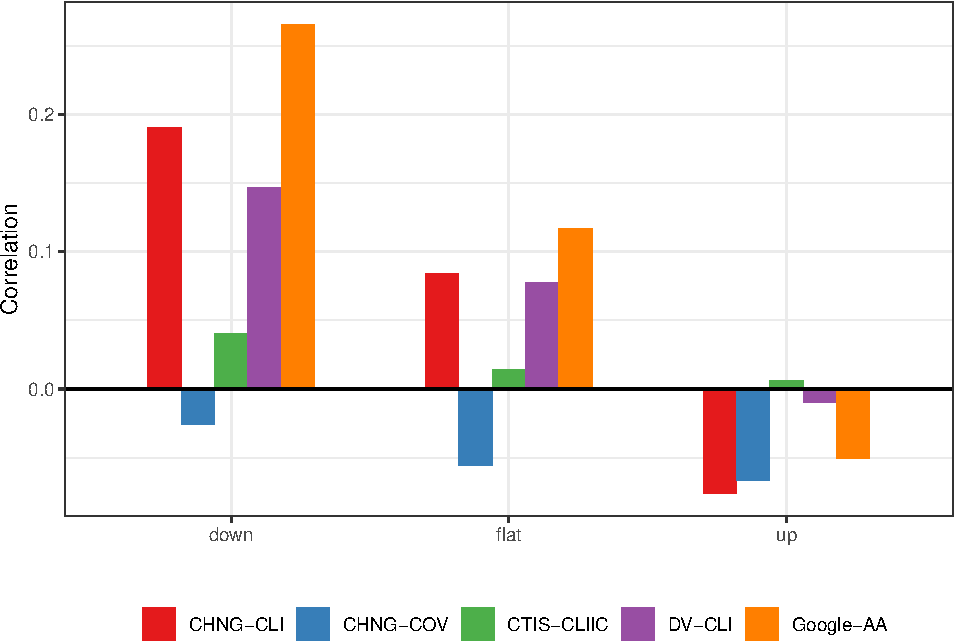
\includegraphics[width=\linewidth]{fig/diff-in-lead-lag-1} \end{center}

\hypertarget{side-figures-in-their-own-scripts}{%
\section{Side figures (in their own
scripts)}\label{side-figures-in-their-own-scripts}}

\begin{center}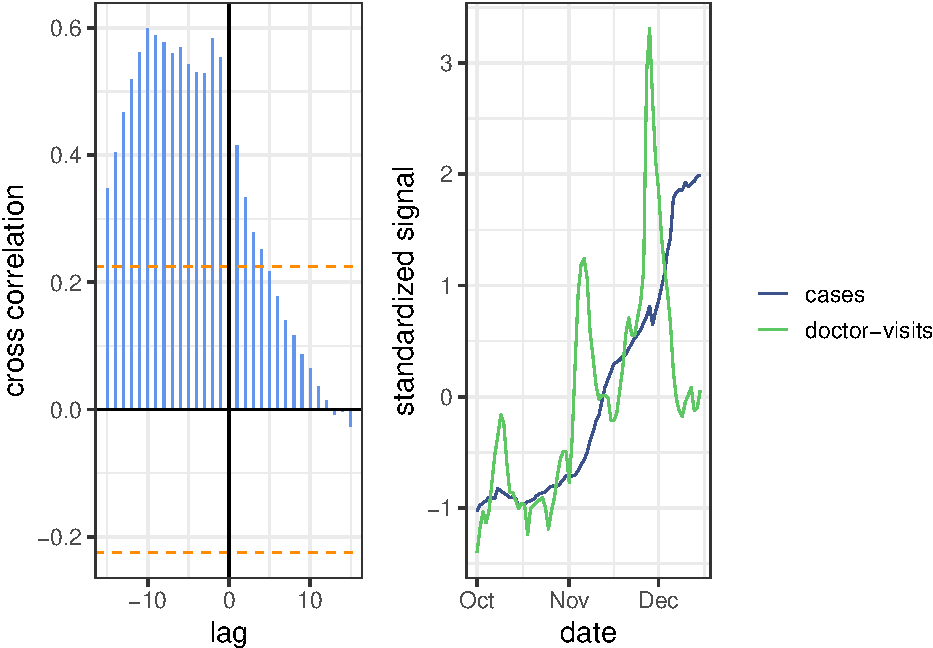
\includegraphics[width=\linewidth]{fig/ccf-dv-finalized-1} \end{center}

\begin{center}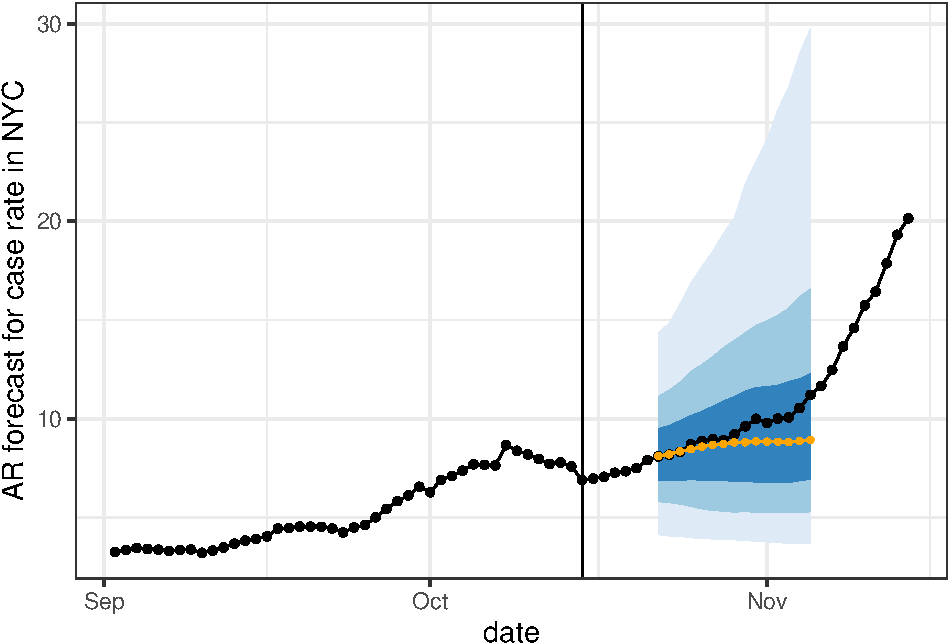
\includegraphics[width=\linewidth]{fig/ny-trajectory-1} \end{center}

\begin{center}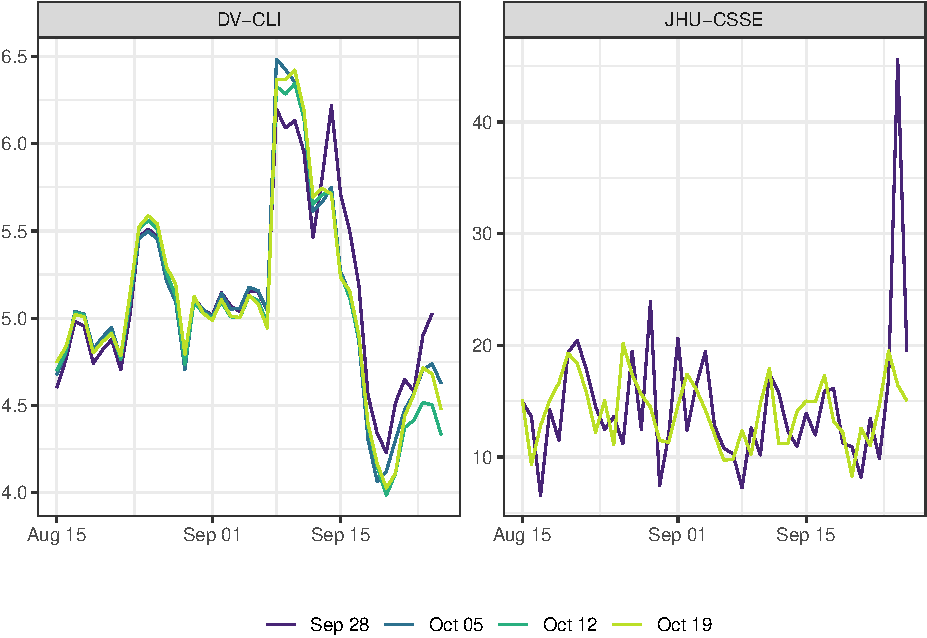
\includegraphics[width=\linewidth]{fig/revisions-dv-jhu-1} \end{center}



%%% Add this line AFTER all your figures and tables
\FloatBarrier

\movie{Type legend for the movie here.}

\movie{Type legend for the other movie here. Adding longer text to show what happens, to decide on alignment and/or indentations.}

\movie{A third movie, just for kicks.}

\dataset{dataset_one.txt}{Type or paste legend here.}

\dataset{dataset_two.txt}{Type or paste legend here. Adding longer text to show what happens, to decide on alignment and/or indentations for multi-line or paragraph captions.}


\bibliography{../../common/covidcast.bib,pnas-materials/pnas-sample.bib}

\end{document}